\chapterhead{3}{Warm Things Cool Down}{Warmth moves from hot to cold}\label{ch3}

Rub your hands together hard for twenty seconds. They warm up. You did not light a fire. The motion of your hands turned into warmth, so rubbing is a way to change motion into warmth.

Warmth can also move on. A cup of warm water on a table loses warmth to the air and the table until it is as cool as the room. The cup's warmth did not disappear. It went to the room, which got a tiny bit warmer.

\begin{center}
\sffamily\small\renewcommand{\arraystretch}{1.5}
\begin{tabular}{@{}p{3.4cm}p{3.7cm}p{3.7cm}@{}}
\toprule
\textbf{Model} & \textbf{What it keeps} & \textbf{What it drops}\\
\midrule
Rubbing as a change & motion becoming warmth & how each rub heats\\
A temperature drop & how much warmth left & where in the room it went\\
A lid & how much warmth it held in & its exact thickness\\
\bottomrule
\end{tabular}
\end{center}

\begin{tryit}{Rub and feel}
Press your palms together and rub them quickly for 20 seconds. Then hold one palm against your cheek. Now try slow rubbing for 20 seconds and compare.\par\medskip
\renewcommand{\arraystretch}{1.6}
\begin{tabular}{|l|c|c|}
\hline
 & \textbf{Fast rub} & \textbf{Slow rub}\\ \hline
\textbf{Warmth (none, little, lots)} & & \\ \hline
\end{tabular}
\end{tryit}

\begin{tryit}{Two cups}
\textbf{You need:} two identical cups, a thermometer in \textdegree C, a clock, warm tap water (never boiling), a lid or plate for one cup.
\begin{enumerate}[leftmargin=1.6em]
\item Pour the same amount of warm tap water into each cup. Put the lid on one.
\item Read both thermometers at the start and every 5 minutes for 20 minutes.
\end{enumerate}
\par\medskip
\renewcommand{\arraystretch}{1.6}
\begin{tabular}{|l|c|c|c|c|c|}
\hline
\textbf{Minutes} & \textbf{0} & \textbf{5} & \textbf{10} & \textbf{15} & \textbf{20}\\ \hline
\textbf{Open (\textdegree C)} & & & & & \\ \hline
\textbf{Lidded (\textdegree C)} & & & & & \\ \hline
\end{tabular}
\end{tryit}
\adult{Use warm tap water only, never water from a kettle or stove. An adult should check the temperature first.}

\begin{worked}{Practice numbers, not from a real test}
Open cup: 46, 41, 37, 34, 31. Drops: 5, 4, 3, 3, total 15. Lidded cup: 46, 43, 41, 39, 38. Drops: 3, 2, 2, 1, total 8.\\
The open cup lost 15 units of warmth and the lidded cup lost 8. The lid slowed the warmth leaving. The difference is $15-8=7$.
\end{worked}

\begin{multix}[hmm]\multixbot[hmm]\tcblower
My hands got warm from rubbing, which means I made warmth from nothing. Free heat! I will build a heater. Is that how it works?
\end{multix}

\trust{We started both cups at the same temperature, used the same amount of water and read them at the same times.}
{The open cup lost more warmth than the lidded cup in every interval, so the lid made the difference.}
{Where in the room the warmth went. The room warms by too little for our thermometer to notice.}

\begin{keepbox}
We turned cooling into a list of readings. \textbf{We kept} \wline[3.4cm] \textbf{and we set aside} \wline[3.4cm].
\end{keepbox}

\clearpage

\begin{puzzle}{Total drop}
A cup reads 50, 44, 40, 37 over three intervals. Total drop \wline[1.6cm]
\end{puzzle}

\begin{puzzle}{Lid or no lid}
Both cups start at 48. After 20 minutes the lidded cup reads 40 and the open cup reads 34. How much more did the open cup lose? \wline[1.6cm]
\end{puzzle}

\begin{puzzle}{From and to}
Write the form before and after.\\
(a) rubbing hands: \wline[2cm] to \wline[2cm]\\
(b) a ball starting down a ramp: \wline[2cm] to \wline[2cm]
\end{puzzle}

\begin{puzzle}{Unfair test}
Ana's lidded cup started at 55 and Ben's open cup at 45. She says lids work better. What is wrong? \wline[6cm]
\end{puzzle}

\begin{puzzle}{Where does it go?}
A hot cup cools on a table. Name two places its warmth goes. \wline[5cm]
\end{puzzle}

\clearpage

\begin{puzzle}{Cold cup}
A cold cup warms from 8 to 14. How many units did it gain? \wline[1.6cm]
\end{puzzle}

\begin{puzzle}{Predict}
Which cools faster, a small cup of warm water or a big one? Say why, then say how you would test it. \wline[6cm]
\end{puzzle}

\begin{puzzle}{Draw the circles}
A cup drops 15 units. Draw a circle for the cup and a circle for the room.
\begin{center}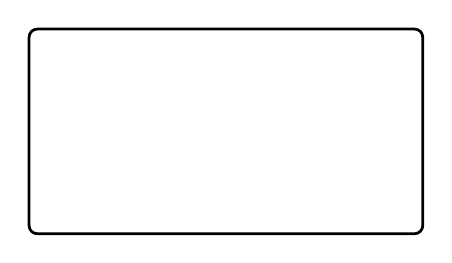
\begin{tikzpicture}\draw[line width=1pt,rounded corners=3pt] (0,0) rectangle (5,2.6); \end{tikzpicture}\end{center}
\end{puzzle}

\begin{puzzle}{Wrap}
A student wrote ``The cold went into the cup.'' Wrap it with a better claim. \wline[6cm]
\end{puzzle}

\begin{puzzle}{Design a keeper}
Say how you would keep a drink warm for an hour, and which readings would show it worked. \wline[6cm]
\end{puzzle}
\clearpage

\thispagestyle{fancy}
\subhead{Cooling record}
Test three ways of keeping water warm: a lid, a cloth wrapped round, a sock. Use the same start and the same cup.\par\medskip
\renewcommand{\arraystretch}{3.0}
\begin{tabularx}{\linewidth}{|>{\sffamily\small\bfseries}p{2.6cm}|X|X|X|X|}
\hline
Cover & Start (\textdegree C) & After 20 min & Drop & Rank \\ \hline
 & & & & \\ \hline
 & & & & \\ \hline
 & & & & \\ \hline
\end{tabularx}

\vspace{8pt}
Which cover kept the warmth best? \wline[7cm]\\[10pt]
How would a repeat make this more trustworthy? \wline[5cm]\\[10pt]
Sketch your cups and show where the warmth escapes.\par\medskip
\begin{tikzpicture}\draw[ink!70,line width=1pt,rounded corners=3pt] (0,0) rectangle (11.4,5.2);\end{tikzpicture}
\clearpage
